% Copyright (c) 2021-10-07 Eclipse Arrowhead Project
%
% This program and the accompanying materials are made available under the
% terms of the Eclipse Public License 2.0 which is available at
% http://www.eclipse.org/legal/epl-2.0.
%
% SPDX-License-Identifier: EPL-2.0

\subsection{Stakeholders}

\begin{figure}[ht!]
  \centering
  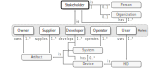
\includegraphics{figures/stakeholder}
  \caption{
    X
  }
  \label{fig:stakeholder}
\end{figure}

\subsection{Entities}

\begin{figure}[ht!]
  \centering
  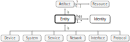
\includegraphics{figures/entity}
  \caption{
    X
  }
  \label{fig:entity}
\end{figure}

\subsection{Devices}

\begin{figure}[ht!]
  \centering
  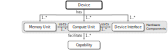
\includegraphics{figures/device}
  \caption{
    X
  }
  \label{fig:device}
\end{figure}

\subsection{Systems}

\begin{figure}[ht!]
  \centering
  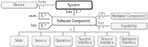
\includegraphics{figures/system}
  \caption{
    X
  }
  \label{fig:system}
\end{figure}

The system has its own identity. A single software artifact can host multiple systems, given that each system is distinct from all others.

\subsection{Services}

\begin{figure}[ht!]
  \centering
  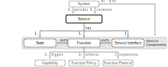
\includegraphics{figures/service}
  \caption{
    X
  }
  \label{fig:service}
\end{figure}

TODO: Explain function invocation. Separate diagram?

\subsection{System-of-Systems}

\begin{figure}[ht!]
  \centering
  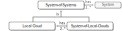
\includegraphics{figures/system-of-systems}
  \caption{
    X
  }
  \label{fig:system-of-systems}
\end{figure}

\subsubsection{Local Clouds}

\begin{figure}[ht!]
  \centering
  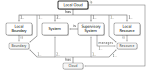
\includegraphics{figures/local-cloud}
  \caption{
    X
  }
  \label{fig:local-cloud}
\end{figure}

\subsubsection{System-of-Local-Clouds}

X

\subsection{Networks}

\begin{figure}[ht!]
  \centering
  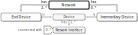
\includegraphics{figures/network}
  \caption{
    X
  }
  \label{fig:network}
\end{figure}

\subsection{Interfaces}

\begin{figure}[ht!]
  \centering
  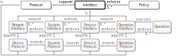
\includegraphics{figures/interface}
  \caption{
    X
  }
  \label{fig:interface}
\end{figure}

TODO: Discussion about difference between interface and service?

\subsection{Policies}

\begin{figure}[ht!]
  \centering
  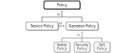
\includegraphics{figures/policy}
  \caption{
    X
  }
  \label{fig:policy}
\end{figure}

\subsection{Protocols}

\begin{figure}[ht!]
  \centering
  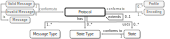
\includegraphics{figures/protocol}
  \caption{
    X
  }
  \label{fig:protocol}
\end{figure}


\subsection{Data}

\begin{figure}[ht!]
  \centering
  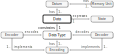
\includegraphics{figures/data}
  \caption{
    X
  }
  \label{fig:data}
\end{figure}